\vfill\null
\columnbreak
\soul{Conceptos de Teletráfico y QoS}
\begin{minipage}{.22\textwidth}
	\begin{tikzpicture}
		\node[draw,circle] (Trafico) at (90:2.2) {Tráfico};
		\node[draw,circle] (Calidad) at (210:2.2) {Calidad};
		\node[draw,circle] (Capacidad) at (330:2.2) {Capacidad};
		\draw[latex'-latex',double] (Trafico) -- node[] {} (Calidad);
		\draw[latex'-latex',double] (Calidad) -- node[] {} (Capacidad);
		\draw[latex'-latex',double] (Capacidad) -- node[] {} (Trafico);
	\end{tikzpicture}
	\begin{itemize}[leftmargin=*]
		\item {\bf QoS (Quality of Service)} (seguridad, calidad...)
		\item {\bf GoS (Grade of Service)} es la calidad que ofrece cada elemento de la red. El GoS de P2P es la QoS.
		\item {\bf Control de tráfico} verifica usuarios conectados a la red usan los servicios que tienen contratado
	\end{itemize}
\end{minipage}

\soul{Introducción teoría de colas}
\begin{minipage}{.22\textwidth}
	$A/B/m/K/N/Z$ Notación de Kendall \\
	(Probabilidades mirar anterior) \\
	a: tráfico observado por el sistema \\
	A: tráfico real ofrecido \\
	$T_o = \lambda \frac{1}{\mu} = T_c + T_p$ Tráfico ofrecido\\
	$B_{LL}$: Congestión en llamdas\\
	$B_{T}$: Congestión en tiempo\\
	$\rho = \frac{T_c}{m}$: Ocupacion media\\
	$\overline{\lambda}$: Tasa efectiva de llegadas\\
	$\overline{N}$: Número medio de usuarios en el sistema\\
	$\overline{Q}$: Número medio de usuarios en cola\\
	$\overline{T}$: Tiempo medio de permanencia en el sistema\\
	$\overline{W}$: Tiempo medio de espera\\
	Media Usuarios servidores: $\overline{N}-\overline{W}$ \\
	$\overline{T} =\overline{W}+\frac{1}{\mu}|$ Fórmula de Little: $\overline{N} =\overline{T}\overline{\lambda}$\\
	$\overline{N} = \overline{Q} + m{\rho}$\\
	$\overline{Q} = \overline{\lambda} \cdot \overline{W} $\\
	$A=\frac{\lambda}{\mu}$ \\
	$B_{LL}=\frac{T_p}{T_o}$ \\
	$T_c=\frac{V_t}{t}$ \\
\end{minipage}

\vfill\null
\columnbreak
\begin{minipage}{.22\textwidth}
	\begin{tabular}{lp{3cm} l}
		$T_0=\frac{1}{\mu}\sum\limits_0^k{\lambda_{i}p_{i}}$                           & $T_c=\frac{1}{\mu}\sum\limits_1^k{\mu_{i}p_{i}} $      \\
		$T_p=\frac{1}{\mu}{\lambda_{k}p_{k}}$                                          & $B_T=\sum_{m}^{k}p_{i} $                               \\
		$\overline{\lambda}=\sum\limits_{0}^{k-1}{\lambda_{i}p_{i}}=\lambda(1-B_{LL})$ & $\overline{N}=\sum\limits_{1}^{k}{{i}p_{i}}$           \\
		$\overline{Q}=\sum\limits_{m+1}^{k}{(i-m)p_i}$                                 & $\overline{T}=\frac{\overline{N}}{\overline{\lambda}}$ \\
		$\overline{W}=\frac{\overline{Q}}{\overline{\lambda}}$                         & $\rho=\frac{\overline{\lambda}{\frac{1}{\mu}}}{m}$     \\
		$\overline{T}=\overline{W}+E[S]$                                               & $\overline{N}=\overline{Q}+m\rho$                      \\
	\end{tabular}
\end{minipage}
\soul{Modelo de Erlang (Pérdidas)}
\begin{minipage}{.22\textwidth}
	M/M/m/m
	\begin{tabular}{lp{3cm} l}
		$\lambda_i=\lambda{\mu_i}=i{\lambda}$ &                                                    \\
		$p_0=\frac{1}{\sum_0^m{A^i}{i!}}$     & $p_n=\frac{\frac{A^n}{n!}}{\sum_0^m{A^i}{i!}}$     \\
		$T_0=\frac{\lambda}{\mu}=A$           & $T_c=A\cdot{p_0}\sum\limits_0^{m-1}\frac{A^i}{i!}$ \\
	\end{tabular}
	$T_c=A(1-p_m)$ \\
	$T_p=A\frac{\frac{A^m}{m!}}{\sum\limits_0^m{\frac{A^i}{i!}}} \hskip 2em T_p=AB_{LL}=\frac{LL_p\frac{1}{\mu}}{T}$ \\ \\
	$B_{LL}=\frac{T_p}{T_o} = \frac{\frac{A^m}{m!}}{\sum\limits_0^m{\frac{A^i}{i!}}} = E_{1,m}(A)$ \\
	$B_T = p_m = B_{LL}$ \\
	$\overline{\lambda} = \lambda{(1-p_m)}$ \\
	$\overline{N} = T_c \hskip 4em \overline{Q} = 0$             \\
	$\overline{W} = 0  \hskip 4em \overline{T} = \frac{1}{\mu}$ \\
	$\rho = \frac{T_c}{m}=\frac{A(1-B_{LL})}{m}$ \\
	$T_{c_i} = A[E_{1,i-1}(A)-E_{1,i}(A)]$: Sel seq. \\
	$E_{1,m} = E_{1,m+1}(A+ATC)$ \\
	ATC: Capacidad por enlace adicional \\
	{\underline{Casos concretos}} \\
	$\cdot M/M/\infty/\infty$ \\
	$p_0=e^{-A} \hskip 1.5em p_n=\frac{A^n}{n!}e^{-A}$ \\
	$B_{LL}=\sum\limits_{m+1}^{\infty}p_i$ \\
	$\cdot M/M/1/1$ \\
	$p_0 = \frac{1}{1+A} \hskip 3em p_1=\frac{A}{1+A}$ \\
\end{minipage}

\soul{Modelo de Engset (Pérdidas)}
\begin{minipage}{.22\textwidth}
	M/M/m/m/N \\
	$\lambda_i = \left \{  \begin{matrix} (N-i) \cdot \lambda \hskip 3em i=0,...,m-1 \\
			0 \hskip 3em \text{resto de casos}\end{matrix}  \right .$ \\
	$\mu_i = \left \{  \begin{matrix} (i\mu) \hskip 3em  i=1,...,m \\
			0 \hskip 3em \text{resto de casos}\end{matrix}  \right .$ \\
	$p_0=\frac{1}{\sum_0^m{\binom{N}{i}{A^i}}}$ \\
	$p_n = {p_0}{A^n}\binom{N}{n}$ \\
\end{minipage}

\vfill\null
\columnbreak

\begin{minipage}{.22\textwidth}
	$T_0={A}\cdot{N}\cdot{p_0}\sum_0^m{\binom{N-1}{i}A^i}$ \\
	$T_c={A}\cdot{N}\cdot{p_0}\sum_0^{m-1}{\binom{N-1}{i}A^i}=\overline{N}$ \\
	$T_p={A}\cdot{N}\cdot{p_0}{\binom{N-1}{m}A^m}$ \\
	$B_{T}=Eng_{1,m}(N+1,A)=p_m$ \\
	$B_{LL}=Eng_{1,m}(N,A)=\frac{\binom{N-1}{m}A^m}{\sum\limits_{i=0}^m{\binom{N-1}{m}A^m}}$ \\
	$T_c=\frac{m{\overline{\lambda}}}{\mu}$ \\
	$\overline{T}=\frac{1}{\mu}$ \\
	$\rho=\frac{T_c}{m}=\frac{\overline{\lambda}}{\mu}$ \\
	$A=\frac{a}{1-a(1-B_{LL})}$ \\
	(Suponemos $B_{LL}$, calculamos A, con esa A calculamos nueva $B_{LL}$ y repetimos hasta que el resultado coverja) \\
	{\underline{Casos concretos}} \\
	$\cdot M/M/1/m/N$ \\
	$p_0=\frac{1}{1+NA} \hskip 1.5em p_n=\frac{NA}{1+NA}$ \\
	$\cdot M/M/m/m/1$ \\
	$p_0 = \frac{1}{1+A} \hskip 3em p_1=\frac{A}{1+A}$ \\
\end{minipage}

\soul{Modelo de Bernoulli}
\begin{minipage}{.22\textwidth}
	Requisito: $N\le{m}$ \\
	$A=\frac{a}{1-a} \hskip 3em {p_0}=\frac{1}{(1+A)^N}$ \\ \\
	$p_n=\frac{\binom{N}{n}{A^n}}{(1+A)^N}=\binom{N}{n}\cdot{a^n}\cdot{(1-a)^{N-m}}$ \\ \\
	$T_0=aN=T_c;T_p=0$ \\
	$B_{LL}=0$ \\
	$B_{T}=a^N$ \\
	$\overline{\lambda}=\lambda{N}{(1-a)}$ \\
	$\overline{N}=a{N}$ \\
	$\overline{T}=\frac{1}{\mu}$ \\
	$\rho=\frac{aN}{m}$ \\
	{\bf \underline{Aproximaciones}} \\
	Engset $->$ Erlang si (N$>>$m) \\
	Engset $->$ Bernoulli si (N$<$2m) con \\
	$B_{LL}=\binom{N-1}{m}{a^m}{(1-a)^{N-1-m}}$ \\
\end{minipage}

\soul{Modelo de Erlang (Espera)}
\begin{minipage}{.22\textwidth}
	M/M/m \\
	$\lambda_i=\lambda$ \\
	$\mu_i = \left \{  \begin{matrix} (i\mu) \hskip 3em  i=1,...,m \\
			m\lambda \hskip 3em m<i\end{matrix}  \right .$ \\
	$p_0 = \frac{1}{\sum_0^m{\frac{A^i}{i!}}+\frac{A^m}{m!}\cdot\frac{A}{m-A}}$ \\ \\
	$p_n = \left \{  \begin{matrix} p_0\frac{A^n}{n!} \hskip 3em 1\le{n}\le{m} \\
			p_0\frac{A^n}{m!m^{n-m}} \hskip 3em m<n\end{matrix}  \right .$ \\
\end{minipage}
\vfill\null
\columnbreak
\begin{minipage}{.22\textwidth}
	$T_0=A=T_c \hskip 3em T_p=0$ \\
	$T_d=A\cdot{\frac{m}{m-A}{p_m}}$ \\
	$B_d=\frac{m}{m-A}{p_m} = E_{2,m}{(A)}$ \\ \\
	$E_{2,m}(A)=\frac{m{E_{1,m}(A)}}{m-A[1-{E_{1,m}(A)}]}$ \\
	$B_T=E_{2,m}(A)$ \\
	$B_{LL}=0$ \\
	$\overline{\lambda}=\lambda$ \\
	$\overline{Q}=\frac{A}{m-A}E_{2,m}(A)$ \\
	$\overline{N}=T_c+\overline{Q}=A+\frac{A}{m-A}E_{2,m}(A)$ \\
	$\overline{T}=\frac{1}{\mu}+\frac{1}{\mu(m-A)}E_{2,m}(A)$ \\
	$\rho=\frac{A}{m}$ \\
	$P(W > t) =E_{2,m}(A) e^{-(1-\rho)m\mu{t}}$ \\
	{\bf \underline{Caso particular: M/M/1}} \\
	$p_0=1-A \hskip 3em p_n=A^n(1-A)$ \\
	$T_d=A^2 \hskip 3em B_d=E_{2,1}(A)=A$ \\
	$\overline{Q}=\frac{A^2}{1-A} \hskip 3em \overline{N}=\frac{A}{1-A}$ \\
	$\overline{W}=\frac{A}{\mu-A} \hskip 3em \overline{T}=\frac{A}{\mu-\lambda}$ \\
	$\rho=A$ \\
	{\bf \underline{Caso particular: M/M/$\infty$}} \\
	$p_0=e^{-A} \hskip 3em p_n=\frac{A^n}{n!}{e^{-A}}$ \\
\end{minipage}
\soul{Modelo de Engset (Espera)}
\begin{minipage}{.22\textwidth}
	M/M/m/N/N \\
	$\lambda_i=(N-1)\lambda \hskip 3em 0\le{i}\le{N}$ \\
	$\mu_i = \left \{  \begin{matrix} (i\mu) \hskip 3em  i=1,...,m \\
			m\mu \hskip 3em m<i\le{N}\end{matrix}  \right .$ \\ \\
	$p_0=\frac{1}{\sum_0^{m-1}\binom{N}{i}A^i+\sum_{m+1}^N\frac{i!}{m!\cdot{m^{i-m}}}{\binom{N}{i}A^i}}$ \\ \\
	$p_n = \left \{  \begin{matrix} \binom{N}{n}A^n{p_0} \hskip 3em  0 \le {n} \le {m} \\
			\frac{n!}{m!m^{n-m}}\binom{N}{n}A^n{p_0} \hskip 3em m\le{n}\le{N}\end{matrix}  \right .$ \\ \\
	$T_0=AN\frac{p_0}{p_0|_{N-1}}=T_C$ \\
	$T_p=0$ \\
	$T_d=ANp_0\sum\limits_m^{N-1}\frac{i!}{m!{m^{i-m}}}\binom{N-1}{i}A^i$ \\
	$B_T=\sum\limits_m^{N}\frac{i!}{m!{m^{i-m}}}\binom{N}{i}A^i{p_0}$ \\
	$B_{LL}=0$ \\
	$B_d=\sum\limits_m^{N-1}\frac{i!}{m!{m^{i-m}}}\binom{N-1}{i}A^i{p_0|_{N-1}}=B_T|_{N-1}$\\ \\
	$Eng_{2,m}(N,A)=\frac{\sum\limits_m^{N-1}\frac{i!}{m!{m^{i-m}}}\binom{N-1}{i}A^i}{\sum\limits_0^{m-1}\binom{N}{i}A^i +\sum\limits_m^{N-1}\frac{i!}{m!{m^{i-m}}}\binom{N-1}{i}A^i}$ \\ \\
\end{minipage}
\vfill\null
\columnbreak
\begin{minipage}{.22\textwidth}
	$\overline{N}=p_0[\sum\limits_{i=1}^{m-1}{i}\binom{N}{i}A^i+\sum\limits_{i=m}^{N}{i}\binom{N}{i}A^i\frac{i!}{m!{m^{i-m}}}]$ \\ \\
	$\overline{Q}=\overline{N}-m+p_0\sum\limits_{0}^{m-1}(m-i)\binom{N}{i}A^i$ \\ \\
	$T_0=T_C=A(N-\overline{N})$ \\
	$\overline{\lambda}=(N-\overline{N})\lambda$ \\
	$\overline{T}=\frac{\overline{N}}{\lambda{(N-\overline{N})}}$ \\ \\
	$\overline{W}=\overline{T}-\frac{1}{\mu}$ \\ \\
	$\rho=\frac{A}{m}(N-\overline{N})$ \\
	$A=\frac{a}{1-a(1+\mu\overline{W})}=\frac{a}{1-\frac{\overline{N}}{N}}$ \\ \\
\end{minipage}


\soul{Redes de Jackson (Abiertas)}
\begin{minipage}{.22\textwidth}
	{\bf Definición} \\
	Los usuarios entran, reciben el servicio y se van.\\
	{\bf Características}
	\begin{itemize}[leftmargin=*]
		\item Los usuarios entran aleatoriamente a la red. (No todos los nodos permitan el acceso).
		\item K sistemas en cola
		\item Cada sistema tiene $m_i$ servidores
		\item Todos los sistemas tienen capacidad ${\infty}$
		\item El tiempo de servicio es una exp. de media ${\frac{1}{\mu_i}}$
		\item Las llegadas del exterior siguen un proceso de Poisson de media $\gamma$
		\item Nodo de entrada aleatorio
	\end{itemize}
\end{minipage}

\begin{minipage}{.22\textwidth}
	{\bf Probabilidades}
	\begin{tabular}{lp{3cm} l}
		{\bf }                           & {\bf }                                                                                                \\  \hline
		$q_{s,i}$                        & {\bf Probabilidad de entrada $(P_s)$}: o de que un usuario llegue al sistema por el nodo i-ésimo.     \\ \hline
		$q_{i,d}$                        & {\bf Probabilidad de salida $(P_d)$}: que un usuario abandone el sistema.                             \\ \hline
		$q_{i,j}$                        & {\bf Probabilidad de salto $(P_j)$}: es decir, que vya de un sistema i a un sistema j. ${q_{ii}\ne0}$ \\ \hline
		$\sum\limits_{i=1}^k{q_{s,i}}=1$ & Todos los usuarios que llegan acceden a un nodo                                                       \\ \hline
		\makecell{$\sum\limits_{j=1}^k{q_{i,j}+q_{i,d}}$                                                                                         \\  $=1$                                                                                       \\ ($1\le{i}\le{k}$)} & Todos los usuarios tienen que salir                                                                   \\ \hline
	\end{tabular}
	Nota: Las redes que cumplen estas propiedades se llaman {\bf REDES DE JACKSON (M / M / $m_i$)} \\
	En este caso concreto:
	\begin{flalign}
		&\begin{aligned}\nonumber
			 & P(n_{1},n_{2},...,n_{m}) = \prod\limits_{i=1}^{k}p_i{(n_i)}
		\end{aligned}&&
	\end{flalign}
	\soul{Teorema de Burke}
	La salida de un sistema M/M/m con llegadas $\gamma$ sigue teniendo tasa $\gamma$ \\
	$F(t)=P_r{\{T\le{t}\}}=1-\sum\limits_0^{\infty}{G_i(t)}$ \\
	$G_i(t)=p_i(t)e^{-\lambda{t}}$ \\
	$\left \{  \begin{matrix} p_i=\frac{\lambda}{i-\mu}p_{i-1} \hskip 3em  1 \le {i} \le {m} \\
			p_i=\frac{\lambda}{m\mu}{p_{i-1}} \hskip 3em m\le{1}\end{matrix}  \right .$ \\ \\
	$F(t)=1-e^{-\lambda{t}}=1-\sum\limits_{0}^{\infty}{p_i{e^{-\lambda{t}}}}$ \\
	$\lambda_i=\gamma{q_{si}}+\sum\limits_{j=1}^{k}{\lambda_j{q_{ji}}} \hskip 3em 1 \le {i} \le {k}$ \\
	$\overline{T}=\sum\limits_{1}^{k}\overline{T}\overline{T_1}$ \\
	$e_i=\frac{\lambda_i}{\gamma}$ \\
\end{minipage}
\vfill\null
\columnbreak
\begin{minipage}{.22\textwidth}
	$\overline{T}\cdot\overline{T_1}=e\overline{T_1}$ \\
	$o_i=e_i\frac{1}{\mu_i}$ \\
	$\overline{T}=\frac{1}{\gamma}\sum_{i=1}^{k}{\lambda_i}{\overline{T_i}}$ \\
	$\overline{T_i}=\frac{1}{\mu_i(1-\rho_i)}=\frac{\overline{N_i}}{\lambda_i}$ \\
	$p_i=\frac{\lambda}{\mu}$ \\
	\soul{Redes cerradas}
	{\bf Definción} \\
	Los usuarios permanecen en el sistema, ni entran ni salen. Población constante.
		{\bf Características}
	\begin{itemize}[leftmargin=*]
		\item Los usuarios ya se encuentran en el sistema
		\item M sistemas. (M / M / m)
		\item Tenemos K usuarios
	\end{itemize}
	\begin{center} \end{center}
\end{minipage}


\begin{minipage}{.22\textwidth}
	{\bf Probabilidades}
	\begin{tabular}{lp{3cm} l}
		{\bf }      & {\bf }                                                                                                \\  \hline
		$q_{s,i}=0$ & {\bf Probabilidad de entrada $(P_s)$}: o de que un usuario llegue al sistema por el nodo i-ésimo.     \\ \hline
		$q_{i,d}=0$ & {\bf Probabilidad de salida $(P_d)$}: que un usuario abandone el sistema.                             \\ \hline
		$q_{i,j}$   & {\bf Probabilidad de salto $(P_j)$}: es decir, que vya de un sistema i a un sistema j. ${q_{ii}\ne0}$ \\ \hline
		\makecell{		$\sum\limits_{i=1}^k{q_{i,j}}=1$                                                                          \\ ($1\le{i}\le{k}$)} & Probabilidad de salto entre nodos del sistema                                                       \\ \hline
		\makecell{$S=$                                                                                                      \\ $\{n_{1},n_{2},...,n_{m} |$ \\ $ n_{i}\ge{0}$\\ $\wedge{\sum\limits_{i=1}^{m}n_i = k}\}$} & No todos los estados son posibles. Estados posibles del sistema                                                                  \\ \hline
	\end{tabular}
\end{minipage}

\soul{Gordon y Newell}
\begin{minipage}{.22\textwidth}
	$P(n_1,n_2,...,n_M)=\frac{1}{G(k,M)}\prod_1^M{P_i(n_i)}$ \\
\end{minipage}
\vfill\null
\columnbreak
\begin{minipage}{.22\textwidth}	
	$G(k,M)=\sum_S{\prod_i^M{p_i(n_i)}}$ \\
	$P(n_1,n_2,...,n_M)=\frac{\prod_1^M{p_i(n_i)}}{\sum{\prod_1^M{p_i(n_i)}}}$ \\
	{\bf Caso particular (más usado)} \\
	M/M/1 \\
	$p_i{(n_i)}=(1-A)A^{n_i}$ \\
	$P(n_1,n_2,...,n_M)=\frac{\prod_1^M{(1-A)A^{n_i}}}{\sum{\prod_{j=1}^M{{(1-A)A^{n_i}}}}}$ \\
	$\frac{1}{\mu_i}=\frac{1}{\mu}$ \\
	$\lambda_i=\sum_{j=1}^M{\lambda_j{p_{ji}}} \hskip 3em i=1,2,...,M$ \\
	Estos sistemas tienen infinitas soluciones del tipo: \\
	$(\lambda_1,\lambda_2,...,\lambda_M)=\alpha(\lambda_1^{'},\lambda_2^{'},...,\lambda_M^{'})$
\end{minipage}

\soul{Algoritmo de valor medio (Lavenberg y Raiser)}
\begin{minipage}{.22\textwidth}
	Recursivo en función de K.\\
	$N_1[k-1]\overbrace{-->}^{\text{lleva a}}T_ 1[k]\overbrace{-->}^{\text{lleva a}}N_1[k]\overbrace{-->}^{\text{lleva a}}\lambda_i[k]$ \\
	$\alpha=\frac{\lambda_i[k]}{\lambda_i^{'}}$ \\
\end{minipage}

\soul{Teorema de llegadas (Lavenberg)}
\begin{minipage}{.22\textwidth}
	"En una red cerrada con k usuarios, la probabilidad de estado percibida por un usuario llegando a un nodo es la que tendría la red si hubiera un usuario menos." \\
	$T_i[k]=\frac{1}{\lambda_i}(\overline{N_i[k-1]} + 1) ->$ Primer paso del proceso recursivo \\
	$N_i[k]=k\frac{\lambda_i^{'}{\overline{T_i[k]}}}{\sum_{j=1}^{M}{\lambda_j^{'}{\overline{T_j[k]}}}} ->$ Segundo paso del p.r. \\
	Lo anterior se repite hasta llegar a la población real del sistema y finalmente: \\
	$\lambda_i[k]=\frac{\overline{N_1[k]}}{\overline{T_1[k]}} = k\frac{\lambda_j^{'}}{\sum_{j=1}^{M}{\lambda_j^{'}{\overline{T_j[k]}}}}$ \\
\end{minipage}

\soul{Sistemas de desbordamiento}
\begin{minipage}{.22\textwidth}
	{\bf Condiciones} \\
	1) $\overline{N}$ bajo \\
	2) V[N]$>$E[N] \\
	3) Para mismo $\overline{N}$,$B_{LL}$ aumenta \\
	Sistemas M/M/m/m \\
	$\text{Sist. Ppal.}\left \{  \begin{matrix} \lambda_{ij}=\lambda               \\
			i=0,...,m-1\text{ y }j=0,...,m^{'} \\
			\lambda_{ij}=0 \text{  resto}\end{matrix}  \right .$ \\ \\
	$\text{Sist. Desbord.}\left \{  \begin{matrix} \lambda_{ij}=\lambda         \\
			i=m\text{ y }j=0,...,m^{'}-1 \\
			\lambda_{ij}=0 \text{  }1<m\end{matrix}  \right .$ \\ \\
\end{minipage}

\vfill\null
\columnbreak
\begin{minipage}{.22\textwidth}
	Sistema Principal: $\mu_{ij}=i\mu$ \\
	Sistema Desbordamiento: $\mu_{ij}=j\mu$ \\
\end{minipage}

\soul{Aproximación de Kosten}
\begin{minipage}{.22\textwidth}
	Supone $lim_\infty{m^{'}}=\infty$ \\
	$p_{ij}=(-1)^j{g_0(m)}\sum\limits_{k=j}^{\infty}\frac{(-A)^k}{k!}\frac{g_k(i)}{g_{k+1}(m)g_k(m)}$ \\
	$g_k(l)=e^{-A}\sum_{i=0}^l{\binom{k+i-l}{i}}\frac{A^{l-i}}{(l-i)!}$ \\
	$g_0(l)=e^{-A}\frac{A^l}{l!}$ \\
	$p_j=\sum_{i=0}^m{p_{ij}}$ \\
	$B_{LL}=\sum_{i=0}^{m^{'}}{p_{j}}$ \\
\end{minipage}

\soul{Wilkinson}
\begin{minipage}{.22\textwidth}
	$E[j]=AB_{LL}=A_d$ \\
	$V[j]=A_d(1-A_d+\frac{A}{1+m+A_d-A})$ \\
	$\lambda_j=\lambda(1-\theta)+j\theta\mu \hskip 3em 0\le{\theta}\le{1}$ \\
	$p_0=(1-\theta)^{A^{'}}$ \\
	$A^{'}=\frac{\lambda}{\mu}\frac{1-\theta}{\theta}$ \\
	$\frac{\lambda}{\mu}=A_d$ \\
	$p_k=\binom{A^{'}+k-1}{k}\theta^k(1-\theta)^{A^{'}}$\\
	$E[j]=A^{'}\frac{\theta}{1-\theta}=A_d$ \\
	$V[j]=A^{'}\frac{\theta}{(1-\theta)^2}=\frac{A_d}{1-\theta}$ \\
	$\alpha=\sum{\alpha_i}$ \\
	$v=\sum{v_i}$ \\
\end{minipage}

\soul{Modelo del tráfico aleatorio equivalente}
\begin{minipage}{.22\textwidth}
	Sólo sirve si buscamos el tráfico perdido por el sistema de desbordamiento \\
	Idea: \\
	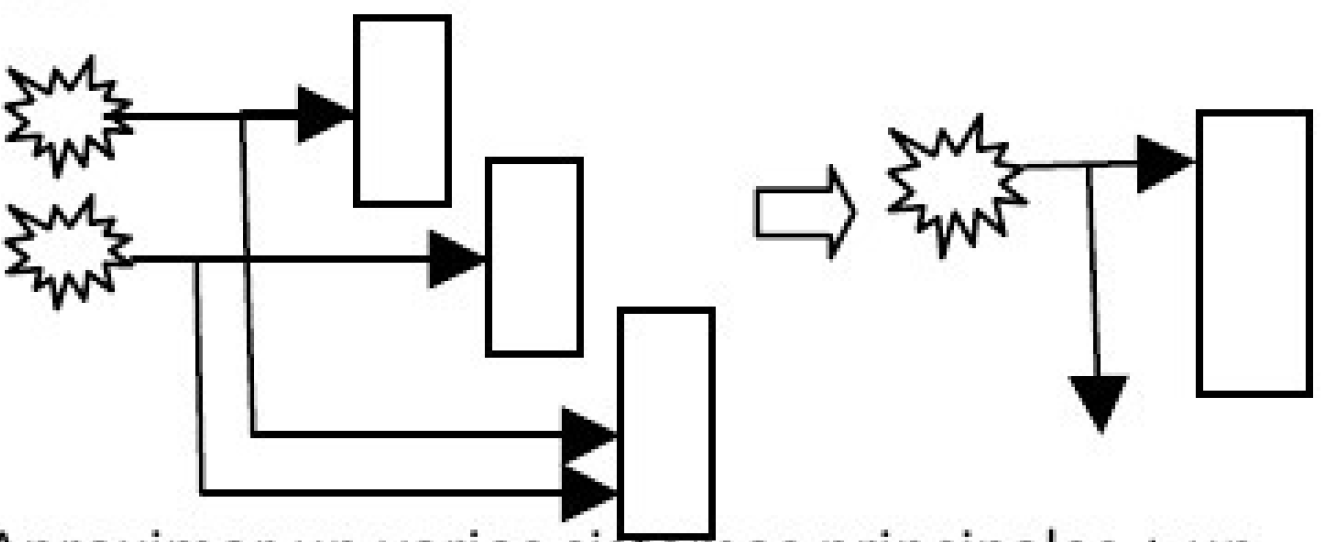
\includegraphics[scale=0.18]{modelotraficoequivalente.png} \\
	Aproximar varios sistemas principales + un sistema de desbordamiento a un único sistema equivalente cuyas pérdidas sean las mismas.\\
	Procedimiento: \\
	{\bf 1)} Obtener $\alpha$ y v\\
	{\bf 2)} Obtener $A_{eq}$ y $m_{eq}$\\ \\
\end{minipage}
\vfill\null
\columnbreak
\begin{minipage}{.22\textwidth}
	Con tablas (abanicos de Wilkinson) \\
	$\alpha=A_{eq}E_{1,m_{eq}}(A_{eq})$ \\
	$v=\alpha(1-\alpha+\frac{A_{eq}}{1+m_{eq}+\alpha-A_{eq}})$\\
	$\alpha_t=\alpha+A$ (Sist. desb. idéntico)\\
	$v_t=v+A$ (Sist. desb. idéntico)\\
	Con aproximación de Rapp: \\
	$A_{eq}=v+3z(z-1)$\\
	$m_{eq}=\frac{A_{eq}}{1-\frac{1}{\alpha+z}}-\alpha-1$ \\
	$z_t=\frac{v_t}{\alpha}$ \\
	{\bf 3)} Obtener $A_{eq}$ y $m^{'}+m_{eq}$ \\
	{\bf 4)} Resolver el sistema equivalente. \\
	Importante: el único parámetro que coincide entre el sistema real y la aproximación es el tráfico perdido, no usar la aproximación para calcular cualquier otra cosa. $T_p=\alpha{B_{LL}}$ \\
	$Go{S_i}=\frac{T_{p_i}}{T_{o_i}}\frac{\alpha^{'}}{\alpha}=(en M/M/m/m)\frac{\alpha_i}{A_i}$
	$GoS_{final}=\prod{G_0{S_i}}$ \\
	$GoS (Sist. desb.) = \frac{T_p}{\alpha_{total}} = \frac{AB_{LL}}{\alpha_{total}}$\\
\end{minipage}

\soul{Sistemas M/G/1}
\begin{minipage}{.22\textwidth}
	No son de nacimiento y muerte.
	No se puede hallar $p_i$ \\
	$\overline{Q}=\lambda{\overline{W}}$ \\
	$\overline{N}=\lambda{\overline{T}}$ \\
	$\overline{T}={\overline{W}}+E[S]$ \\
	$\overline{W}={\overline{W_0}}+{\overline{W_1}}$ \\
	$R[S]=\frac{E[S^2]}{2E[S]}$ \\
	$\overline{W_0}=R[S]\rho=\sum\frac{\lambda_i{E[S_i^2]}}{2}$ (Con varios) \\
	$\overline{W_1}=\overline{Q}E[S]$ \\
	$\overline{W}=\frac{\lambda{E[S^2]}}{2(1-\rho)}$ \\
	$\overline{Q}=\frac{\lambda^2{E[S^2]}}{2(1-\rho)}$ \\
	$\overline{T}=\frac{\lambda{E[S^2]}}{2(1-\rho)}+E[S]$ \\
	$\overline{N}=\frac{\lambda^2{E[S^2]}}{2(1-\rho)}+\rho$ \\
	{\bf Fórmulas de Pollaczek-Khinthine} \\
	$C_S^2=\frac{V[S]}{E^2[S]}$ \\
	$\overline{N}=\rho+\frac{\rho^2}{2(1-\rho)}{(1+C_S^2)}$ \\
	$\overline{Q}=\frac{\rho^2}{2(1-\rho)}{(1+C_S^2)}$ \\
	{\bf Fórmulas de Takácks} \\
	$E[W^2]=2\overline{W^2}+\frac{\lambda{E[S^3]}}{3(1-\rho)}$ \\
	$E[T^2]=E[W^2]+\frac{E[S^2]}{1-\rho}$ \\
	$E[S^2]=E^2[S](1+C_S^2)$ \\
	$E[S^3]=E^3[S](1+C_S^2)(1+2C_S^2)$ \\
\end{minipage}
\vfill\null
\columnbreak
\soul{Sistemas M/G/1 con prioridades}
\begin{minipage}{.22\textwidth}
	P clases en la población. \\
	$\lambda_i$: tasa de llegadas de la clase i-ésima \\
	$E[S_i]$: tiempo medio de servicio de la clase i-ésima \\
	$\rho_i=\lambda_i{E[S_i]} \hskip 2em E[S^2]=V[S]+E^2[S]$ \\
	$\lambda=\sum\limits_{i=1}^P{\lambda_i}$ \\
	$E[S]=\sum_{i=1}^P{\frac{\lambda_i}{\lambda}}E[S_i]$ (También vale para momento orden 2) \\
	$\rho=\sum\limits_{i=1}^P{\rho_i}=\lambda{E[S]}$ \\
	{\bf Teorema de conservación} \\
	Para una disciplina conservativa y sin desalojo se cumple: \\
	$\sum\limits_{i=1}^P{\rho_i}{\overline{W_i}}=\frac{\rho\overline{W_0}}{1-\rho}$ \\
	La disciplina de cola típica en estos sistemas es HOL.
		{\bf HOL (Head of line)} \\
	Cuando un usuario llega al sistema, no se pone el último, se pone inmediatamente después del último usuario de prioridad menor o igual a la suya. \\
	$\overline{W_r^0}$: tiempo medio al desalojo del servidor \\
	$\overline{W_r^1}$: tiempo medio en servir a los que me preceden al llegar \\
	$\overline{W_r^2}$: tiempo medio en servir a los más prioritarios durante la espera \\
	$\overline{W_r}=\overline{W_r^0}+\overline{W_r^1}+\overline{W_r^2}$ \\
	$\overline{W_r^0}=\sum\limits_{i=1}^P\frac{\lambda_i{E[S_i^2]}}{2}$ \\
	$\overline{W_r^1} =\sum\limits_{i=1}^r{\rho_i \overline{W_i}}$ \\
	$\overline{W_r^2} =\sum\limits_{i=1}^{r-1}{\rho_i \overline{W_r}}$ \\
	$\overline{W_r}=\sum\limits_{i=1}^P\frac{\lambda_i{E[S_i^2]}}{2}+\sum\limits_{i=1}^r{\rho_i \overline{W_i}}+\sum\limits_{i=1}^{r-1}{\rho_i \overline{W_r}}$ \\
	Esto da lugar a un sistema de ecuaciones triangular que, resuelto empezando por la clase más prioritaria, da lugar a la fórmula de Cobham.\\
	{\bf Fórmula de Cobham} \\
	$\overline{W_r}=\frac{\overline{W_0}}{(1-\sum_{i=1}^{r-1}{\rho_i})(1-\sum_{i=1}^{r}{\rho_i})}$ \\
\end{minipage}

\vfill\null
\columnbreak
\begin{minipage}{.22\textwidth}
	{\bf Función de costes} \\
	$\sum_{i=1}^P{C_i}{\overline{W_i}}$, asignamos prioridad de manera que: \\
	$\frac{C_1}{\rho_1} > \frac{C_2}{\rho_2} > ... > \frac{C_p}{\rho_p}$ \\
\end{minipage}
\soul{Anexo}
\begin{minipage}{.22\textwidth}
	{\bf Fórmula de Engset} \\
	$Eng_{1,m}(N,A)=\frac{\binom{N-1}{m}A^m}{\sum_0^m{\binom{N-1}{i}A^i}}$ \\
\end{minipage}

\soul{Notación de Kendall}
\begin{minipage}{.22\textwidth}
	A/B/m/K/N/Z \\
	{\bf A: Patrón de llegadas}
	\begin{itemize}[leftmargin=1em]
		\item G: Tiempo entre llegadas con distribución General
		\item $H_k$: Distribución de tiempo entre llegadas para k etapas de tipo hiperexponencial.
		\item $E_k$: Distribución de tiempos entre llegadas de tipo Erlang-K.
		\item M: Distribución de tiempos entre llegadas de tipo exponencial
		\item D: Distribución de tiempos entre llegadas de tipo determinista
	\end{itemize}
	{\bf B: Patrón/Tiempo de servicio}
	\begin{itemize}[leftmargin=1em]
		\item Idem al Patrón de llegadas
	\end{itemize}
	{\bf m: Número de servidores disponibles} \\
	{\bf K: Disciplina de la línea de espera}
	\begin{itemize}[leftmargin=1em]
		\item FIFO (si es FIFO el valor se omite)
		\item LIFO
		\item SIRO (selección aleatoria de clientes)
		\item PRI (servicio por prioridad)
	\end{itemize}
	{\bf N: Capacidad del sistema }
	\begin{itemize}[leftmargin=1em]
		\item Si es infinita se omite
	\end{itemize}
	{\bf Z: tamaño de la población}
	\begin{itemize}[leftmargin=1em]
		\item Si es infinita se omite
	\end{itemize}
\end{minipage}
\vfill\null
\columnbreak
\soul{Modelo de Erlang}
\begin{minipage}{.22\textwidth}
	\begin{itemize}[leftmargin=*]
		\item Población infinita
		\item Tasa de llegada $\lambda$
		\item Tiempo de servicio $->$ distribución exponencial de media $\frac{1}{\mu}$
		\item Los usuarios que completan su llamada vuelven al sistema
		\item Hay m servidores
		\item Capacidad del sistema m
		\item No hay cola de espera
		\item Las llamadas no completadas no se intentan
	\end{itemize}
\end{minipage}


\soul{Modelo de Engset}
\begin{minipage}{.22\textwidth}
	\begin{itemize}[leftmargin=*]
		\item El número de fuentes es finito N
		\item Tasa de llegada $\lambda$ Comportamiento independiente del resto y estado del sistema.
		\item Tiempo de servicio $->$ distribución exponencial de media $\frac{1}{\mu}$
		\item Los usuarios que completan su llamada vuelven al sistema
		\item m servidores en el sistema
		\item No existen posiciones de espera (si no es atendida se abandona)
		\item No existen reintento de llamdas
	\end{itemize}
\end{minipage}

\soul{Modelo de Bernoulli}
\begin{minipage}{.22\textwidth}
	\begin{itemize}[leftmargin=*]
		\item El número de fuentes es finito N
		\item Tasa de llamadas cte. ($\lambda$). Comportamiento independiente del resto y estado del sistema.
		\item Tiempo de servicio $->$ distribución exponencial de media $\frac{1}{\mu}$
		\item Los usuarios que completan su llamada vuelven al sistema
		\item Hay m servidores, superior al nº de fuentes $->$ No existe el rechazo de llamadas
	\end{itemize}
\end{minipage}